
\documentclass[11pt,a4paper]{article}
\usepackage[margin=1in]{geometry}
\usepackage{graphicx}
\usepackage{booktabs}
\usepackage{hyperref}
\usepackage{caption}
\captionsetup{font=small}
\title{Exploratory Data Analysis of EV Battery Charging Sessions}
\author{Generated by ChatGPT}
\date{22 April 2025}

\begin{document}
\maketitle

\section{Introduction}
Electric vehicles (EVs) rely on lithium–ion batteries whose longevity is highly sensitive to charging habits and environmental conditions.  
This technical report explores 1000 recorded charging sessions to uncover patterns that influence battery health, efficiency, and degradation.

\section{Methods}
Raw session logs were inspected for missing values (none found) and obvious sensor errors.  
Numeric attributes were standard–scaled (z‑scores) and the resulting cleaned dataset is available for download:  
\href{run:ev_battery_charging_data_scaled.csv}{ev\_battery\_charging\_data\_scaled.csv}.

\section{Descriptive Statistics}
\begin{center}
\begin{tabular}{lrrrrrrr}
\toprule
Feature & Mean & Std & Min & 25\% & 50\% & 75\% & Max \\
\midrule
SOC (%) & 54.12 & 26.29 & 10.42 & 31.24 & 54.71 & 76.99 & 99.97 \\
Voltage (V) & 3.85 & 0.2 & 3.5 & 3.67 & 3.86 & 4.03 & 4.2 \\
Current (A) & 55.22 & 26.16 & 10.0 & 33.52 & 55.06 & 78.32 & 99.8 \\
Battery Temp (°C) & 29.81 & 5.73 & 20.01 & 24.84 & 29.69 & 34.75 & 39.99 \\
Ambient Temp (°C) & 24.88 & 5.74 & 15.0 & 19.9 & 24.89 & 29.8 & 34.95 \\
Charging Duration (min) & 69.85 & 28.92 & 20.62 & 44.94 & 69.04 & 93.99 & 119.94 \\
Degradation Rate (%) & 10.02 & 2.7 & 4.1 & 8.01 & 10.03 & 12.07 & 16.04 \\
Efficiency (%) & 98.0 & 0.54 & 96.79 & 97.59 & 97.99 & 98.4 & 99.18 \\
Charging Cycles & 556.56 & 263.76 & 101.0 & 317.75 & 571.0 & 786.0 & 999.0 \\
Optimal Charging Duration Class & 1.19 & 0.75 & 0.0 & 1.0 & 1.0 & 2.0 & 2.0 \\
\bottomrule
\end{tabular}
\end{center}

\section{Exploratory Visualisations}
Figures~\ref{fig:soc}--\ref{fig:ambient} provide a visual tour of the dataset.

\begin{figure}[h]
 \centering
 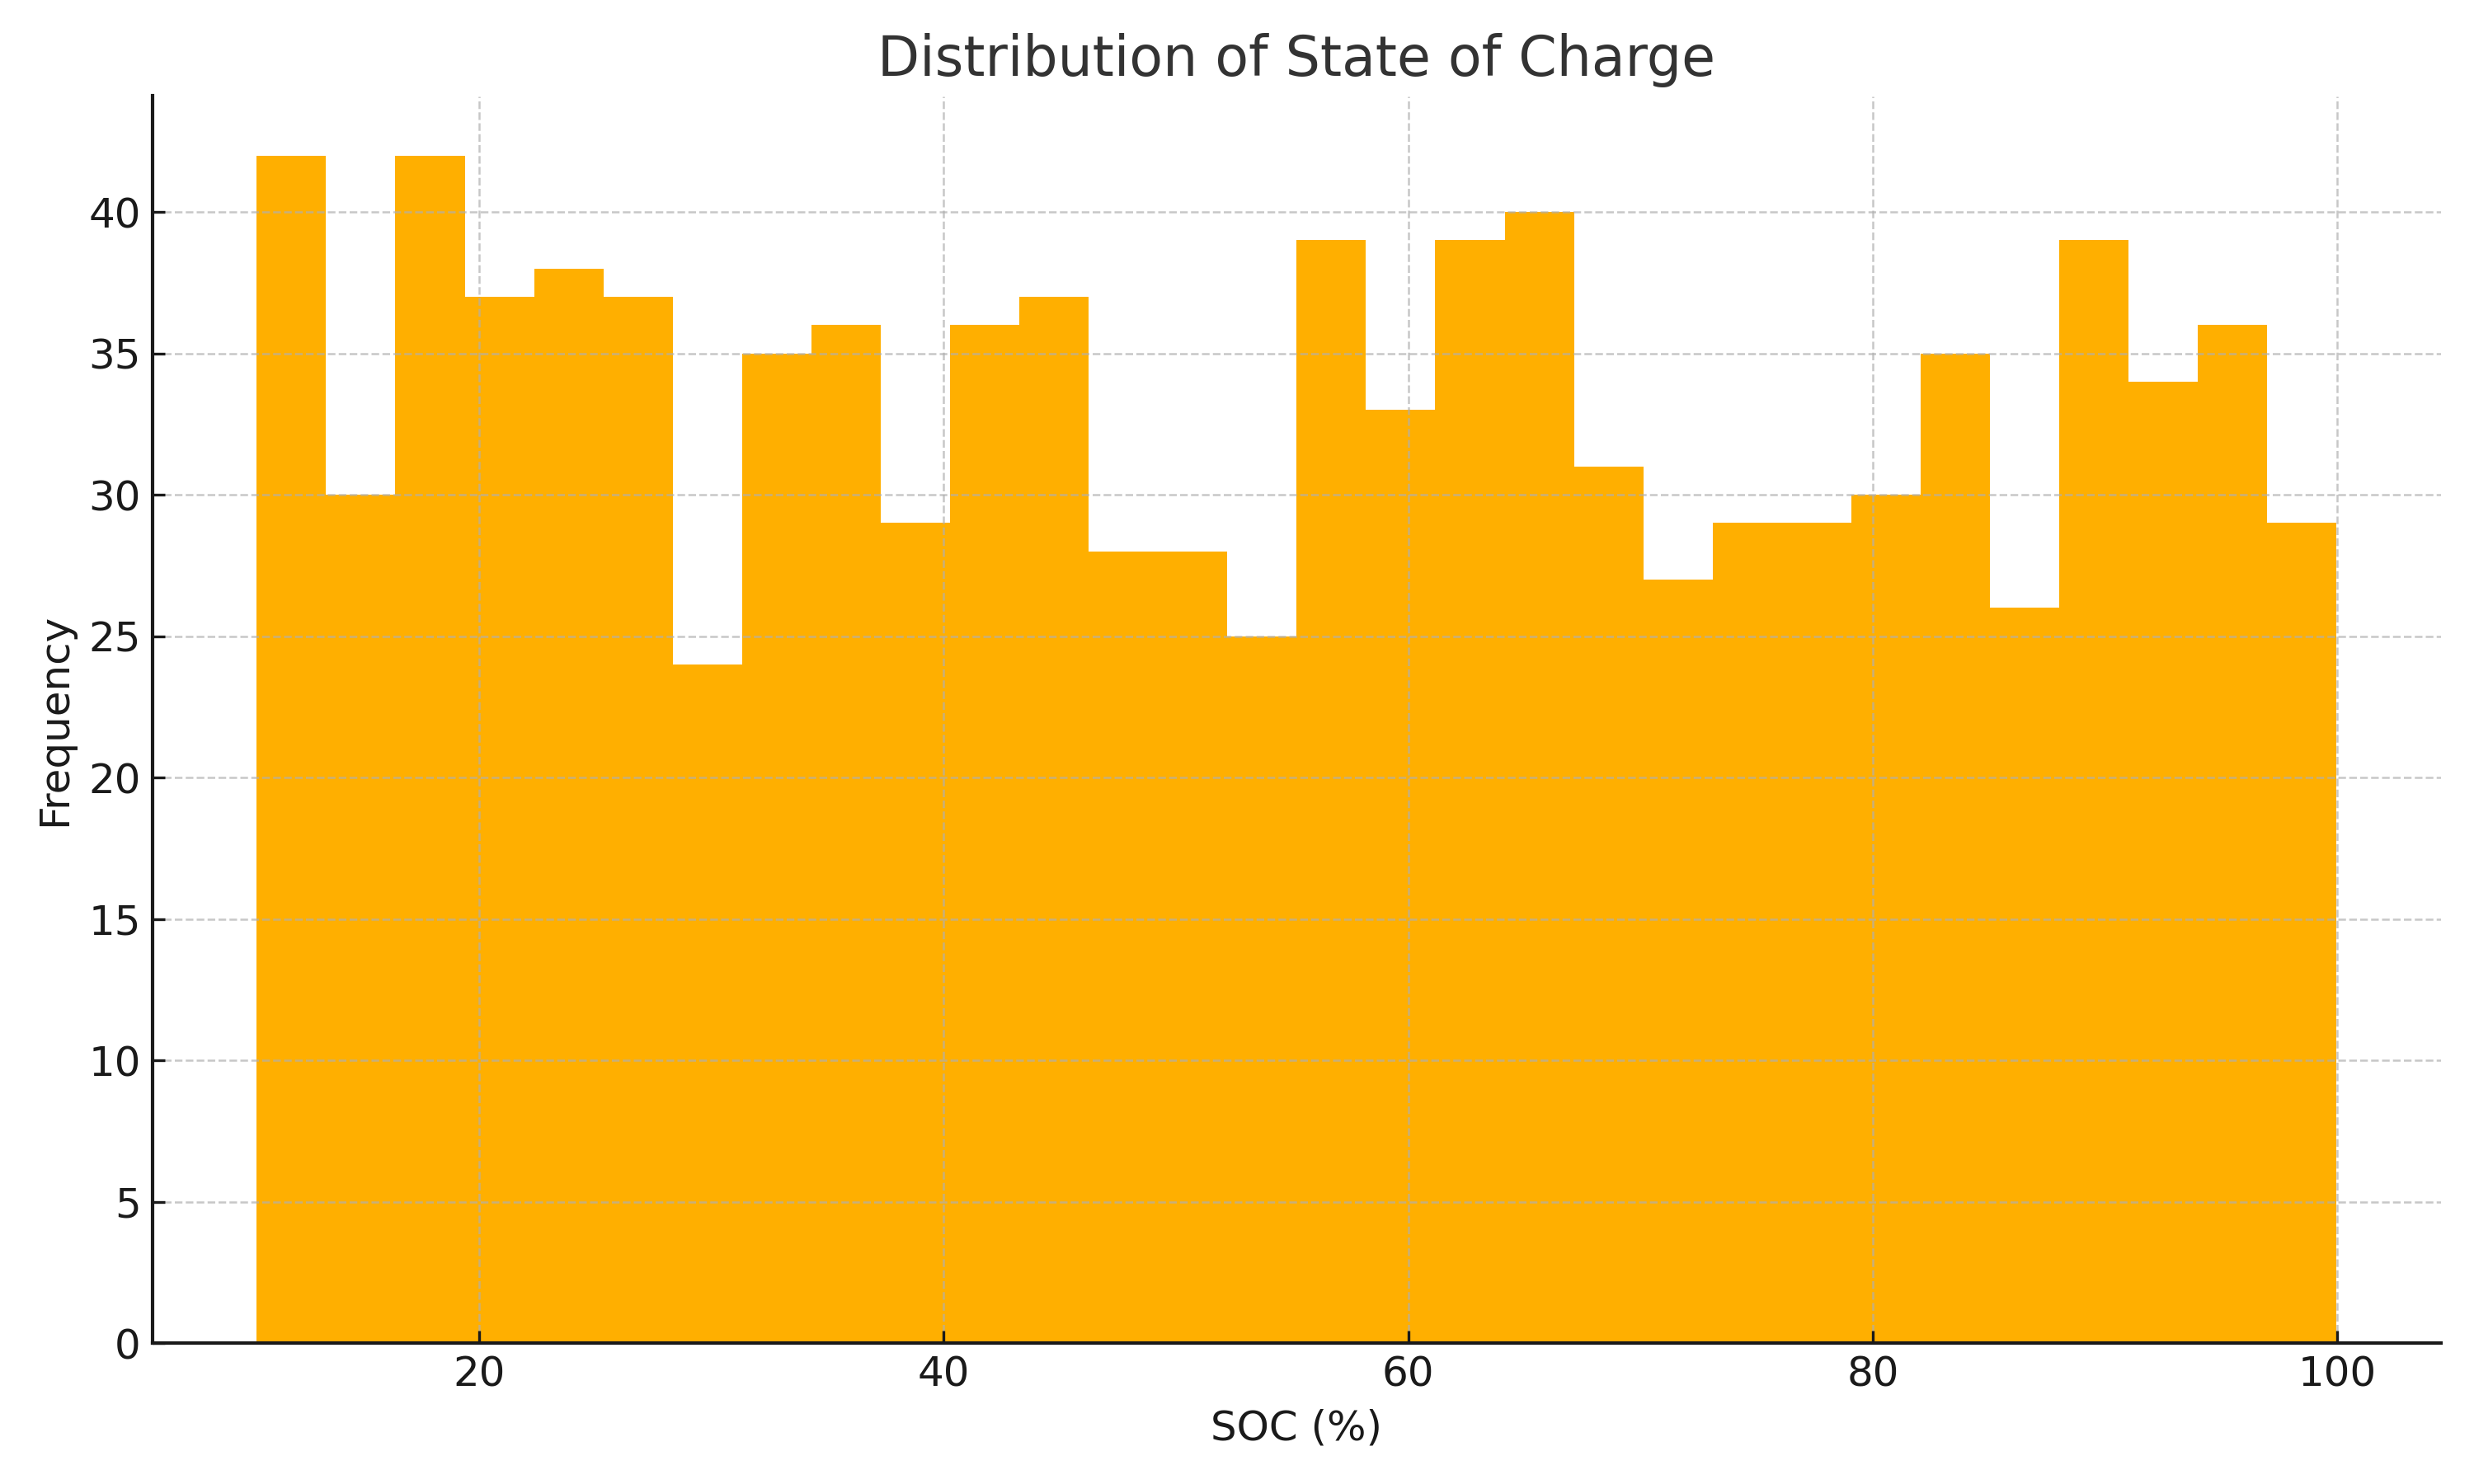
\includegraphics[width=0.7\textwidth]{fig_soc_hist.png}
 \caption{Distribution of State of Charge}
 \label{fig:soc}
\end{figure}

\begin{figure}[h]
 \centering
 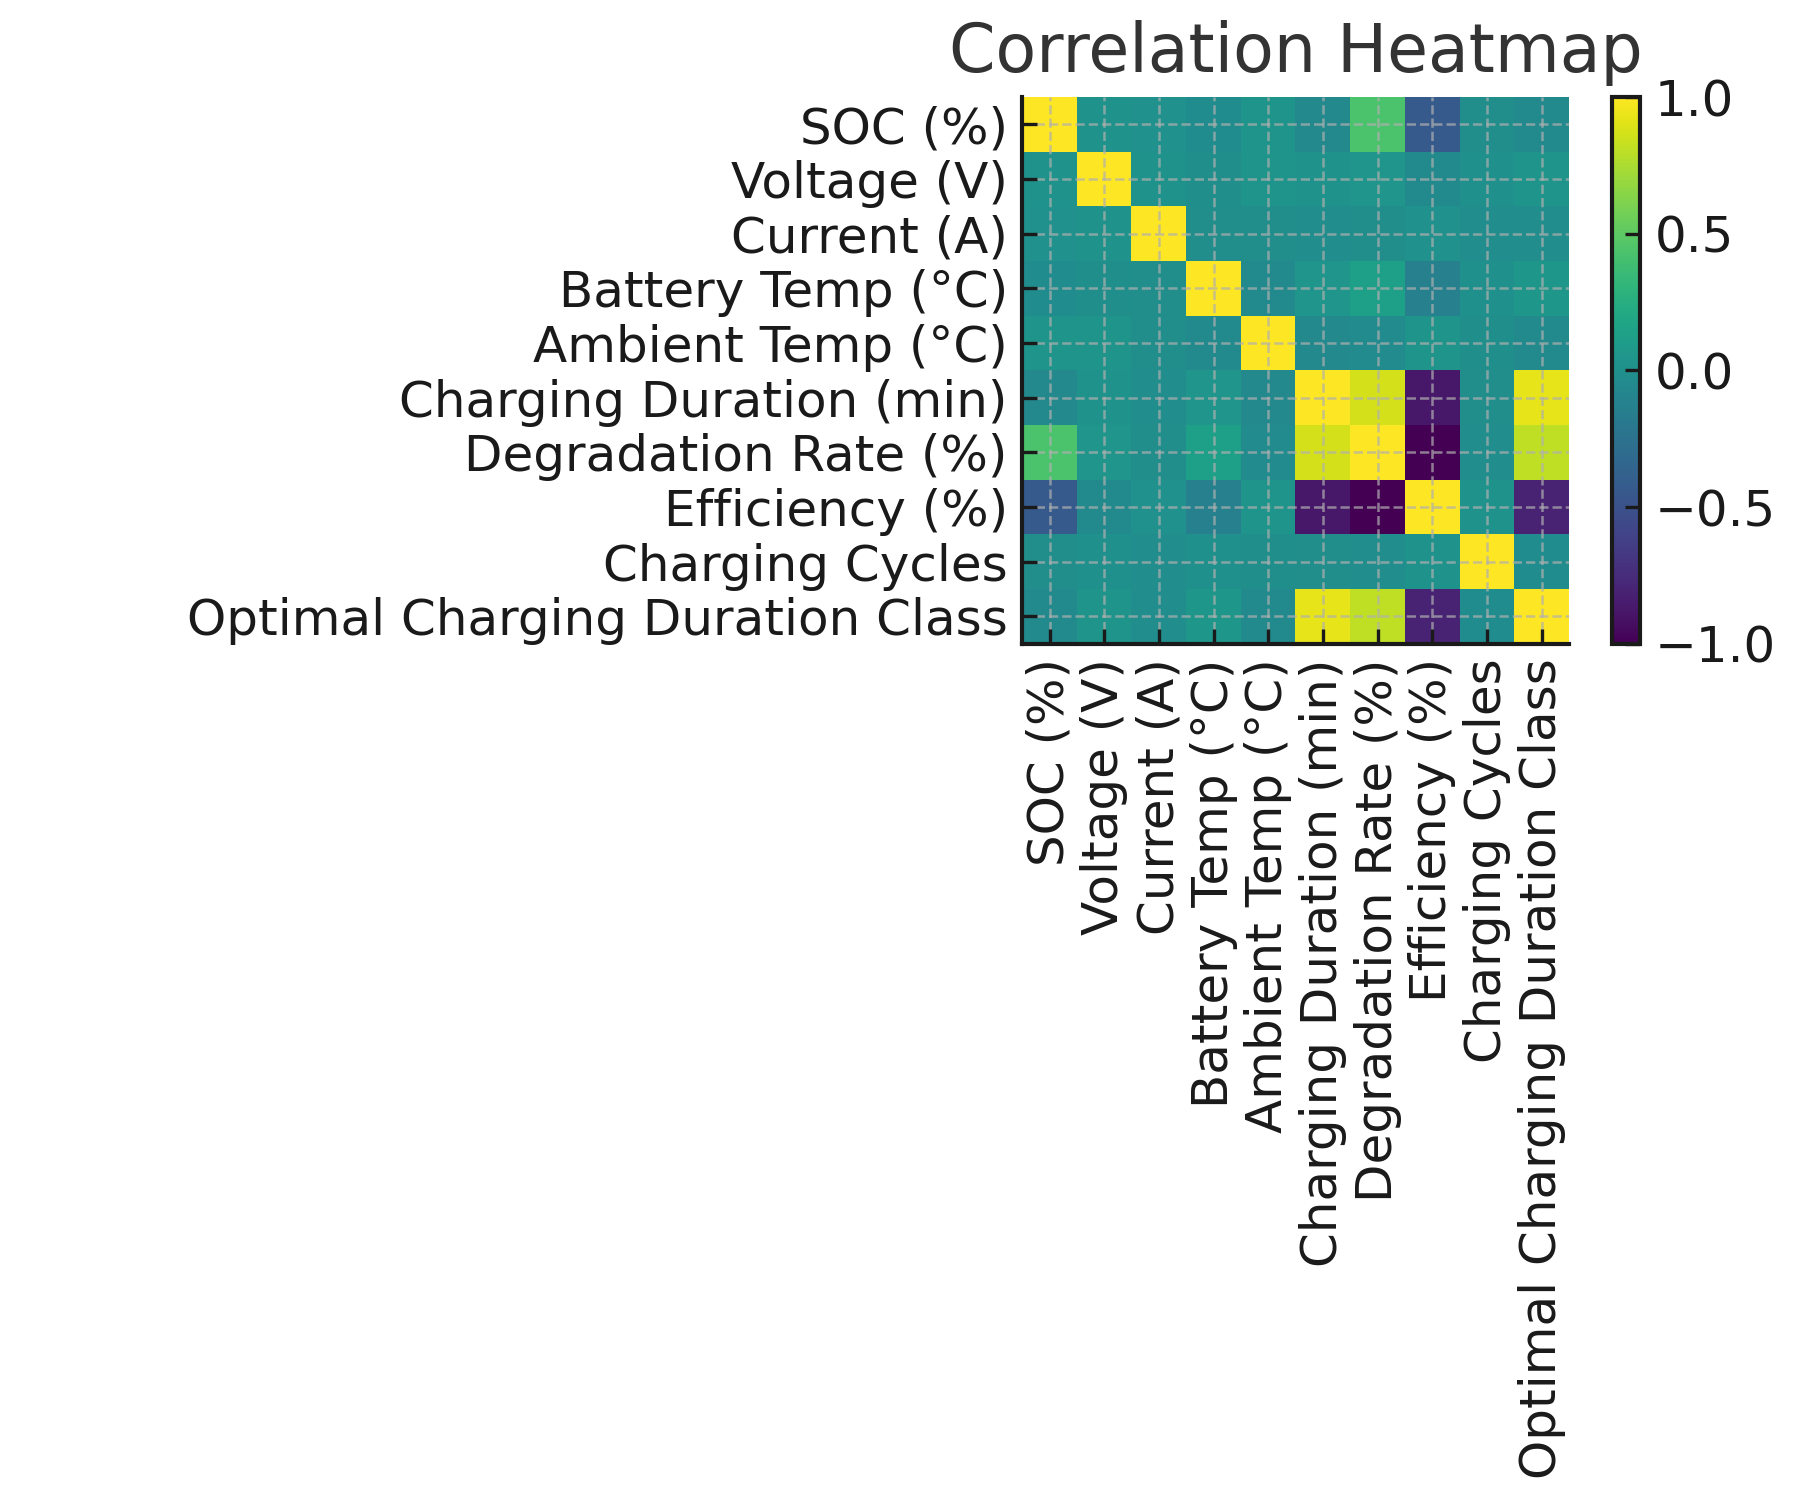
\includegraphics[width=0.7\textwidth]{fig_corr_heat.png}
 \caption{Pearson correlation heatmap of numeric attributes}
 \label{fig:heat}
\end{figure}

\begin{figure}[h]
 \centering
 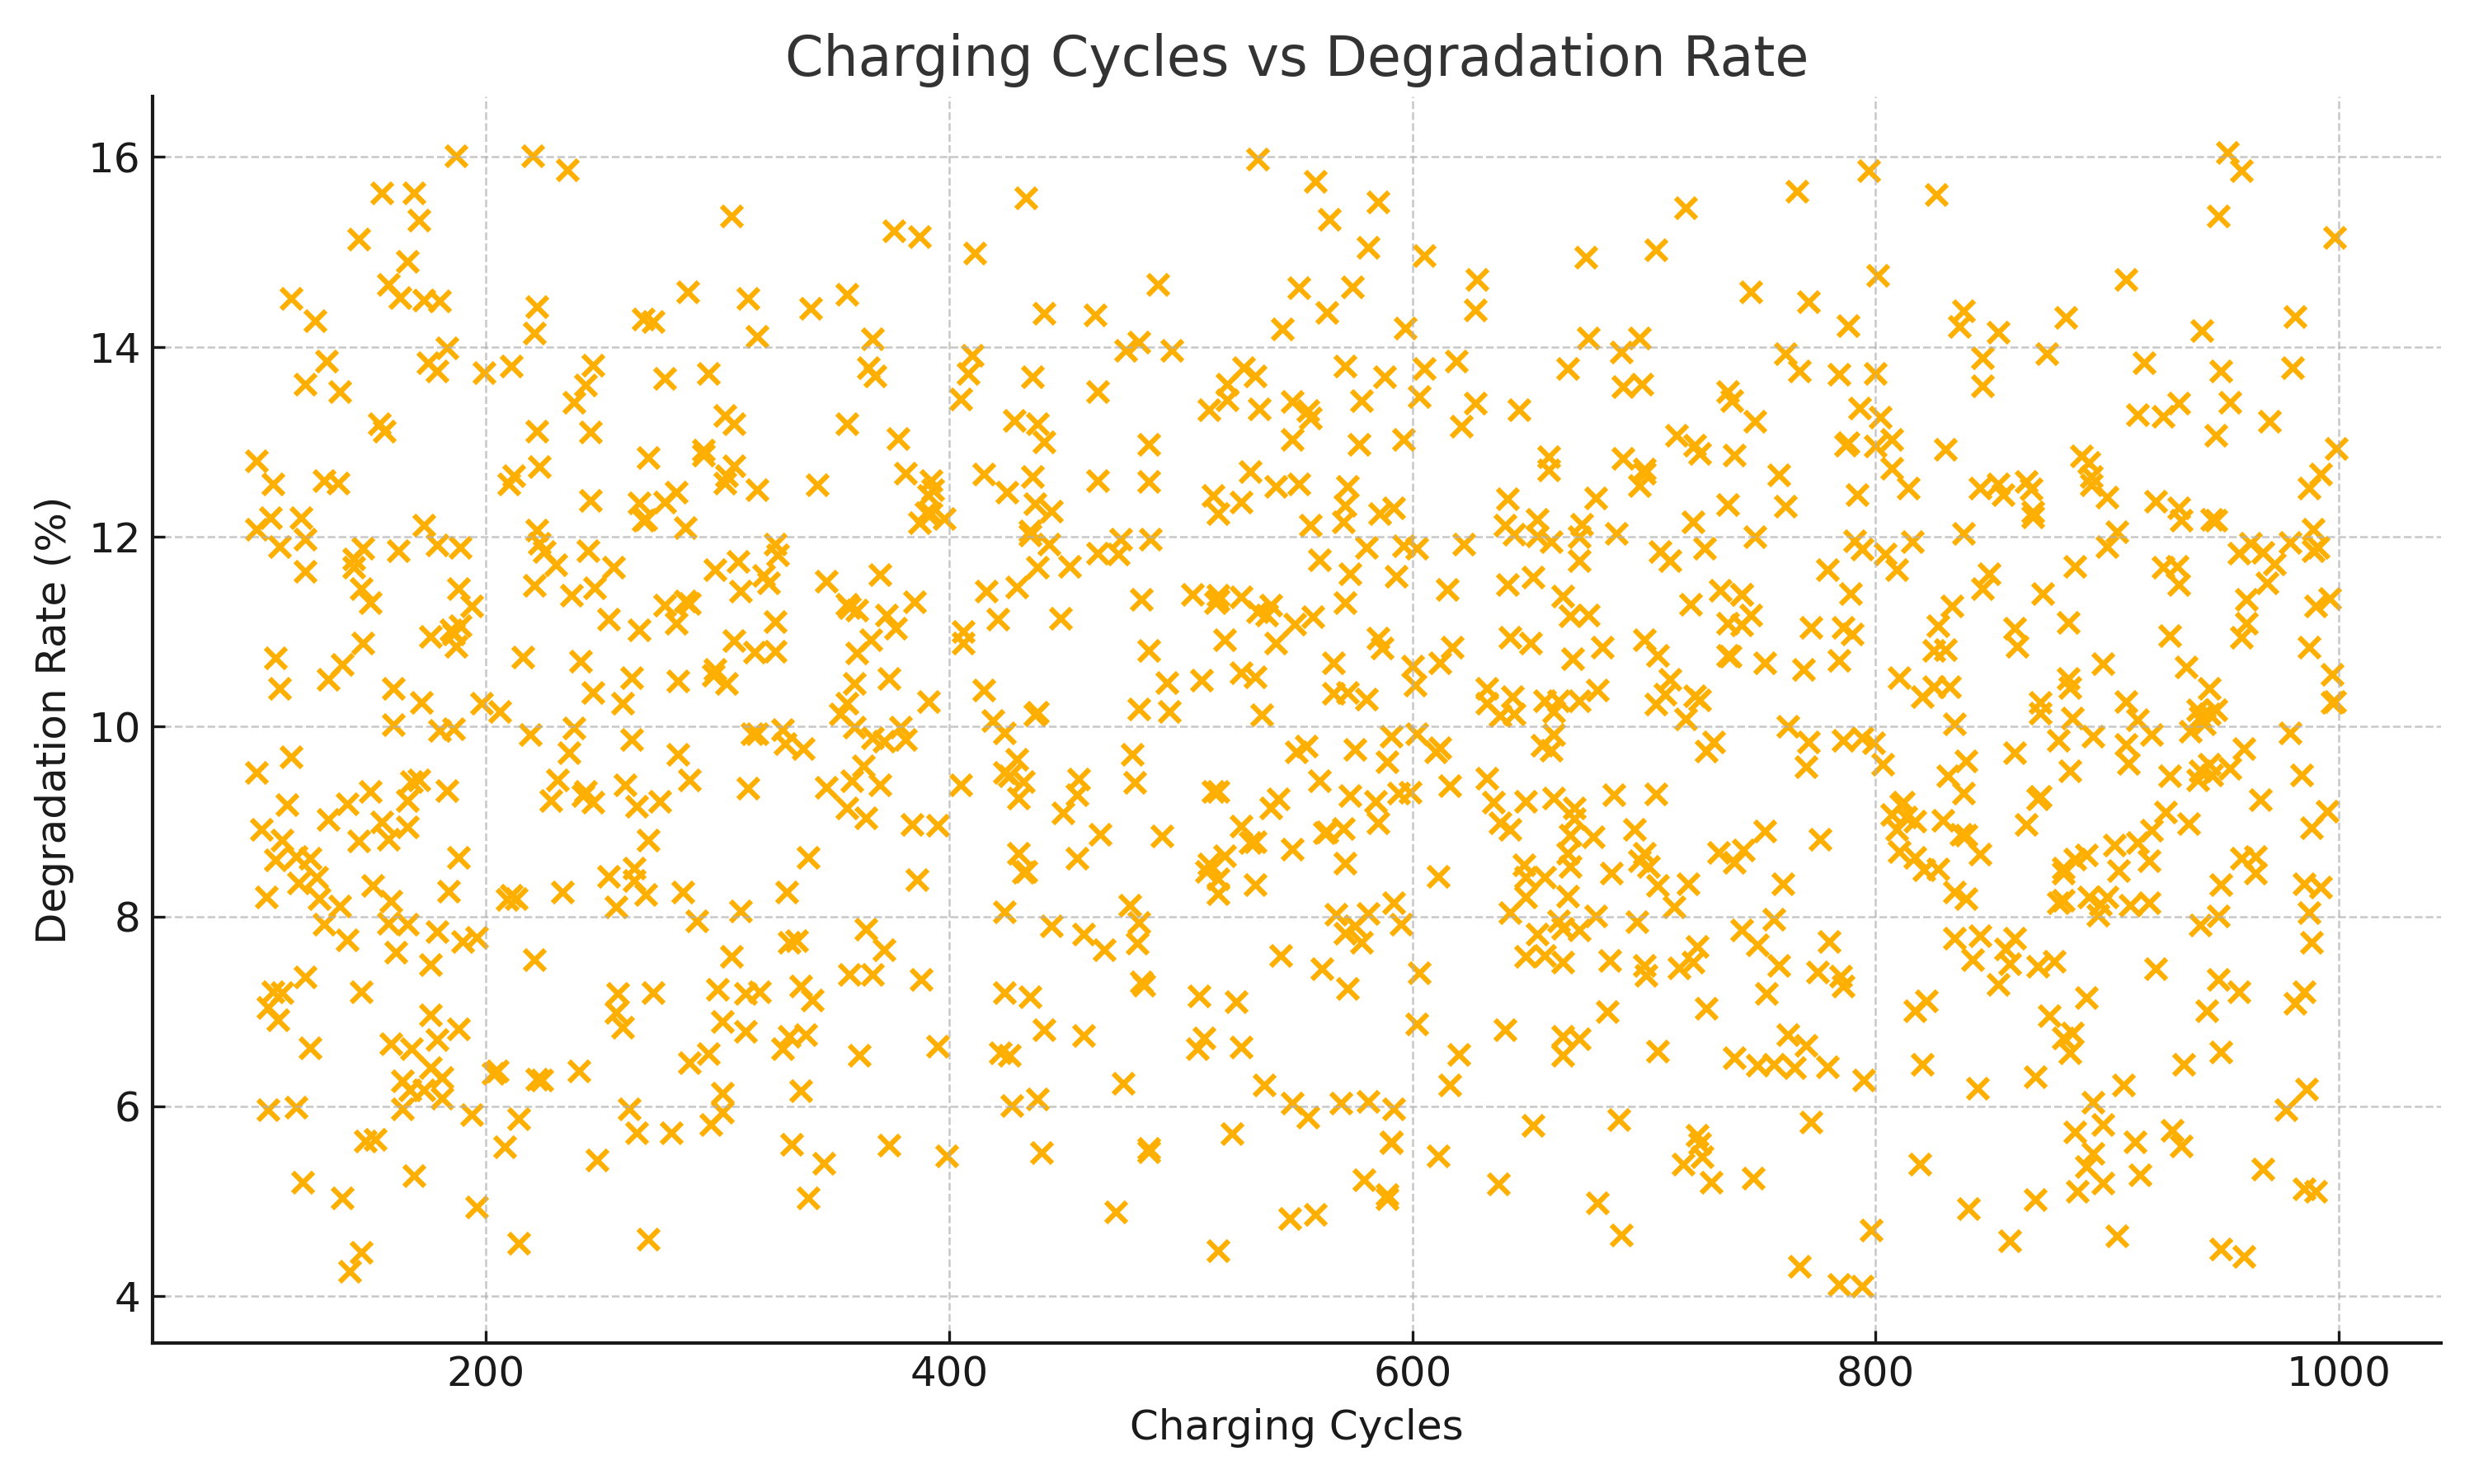
\includegraphics[width=0.7\textwidth]{fig_cycles_deg.png}
 \caption{Charging cycles versus degradation percentage}
 \label{fig:cycles}
\end{figure}

\begin{figure}[h]
 \centering
 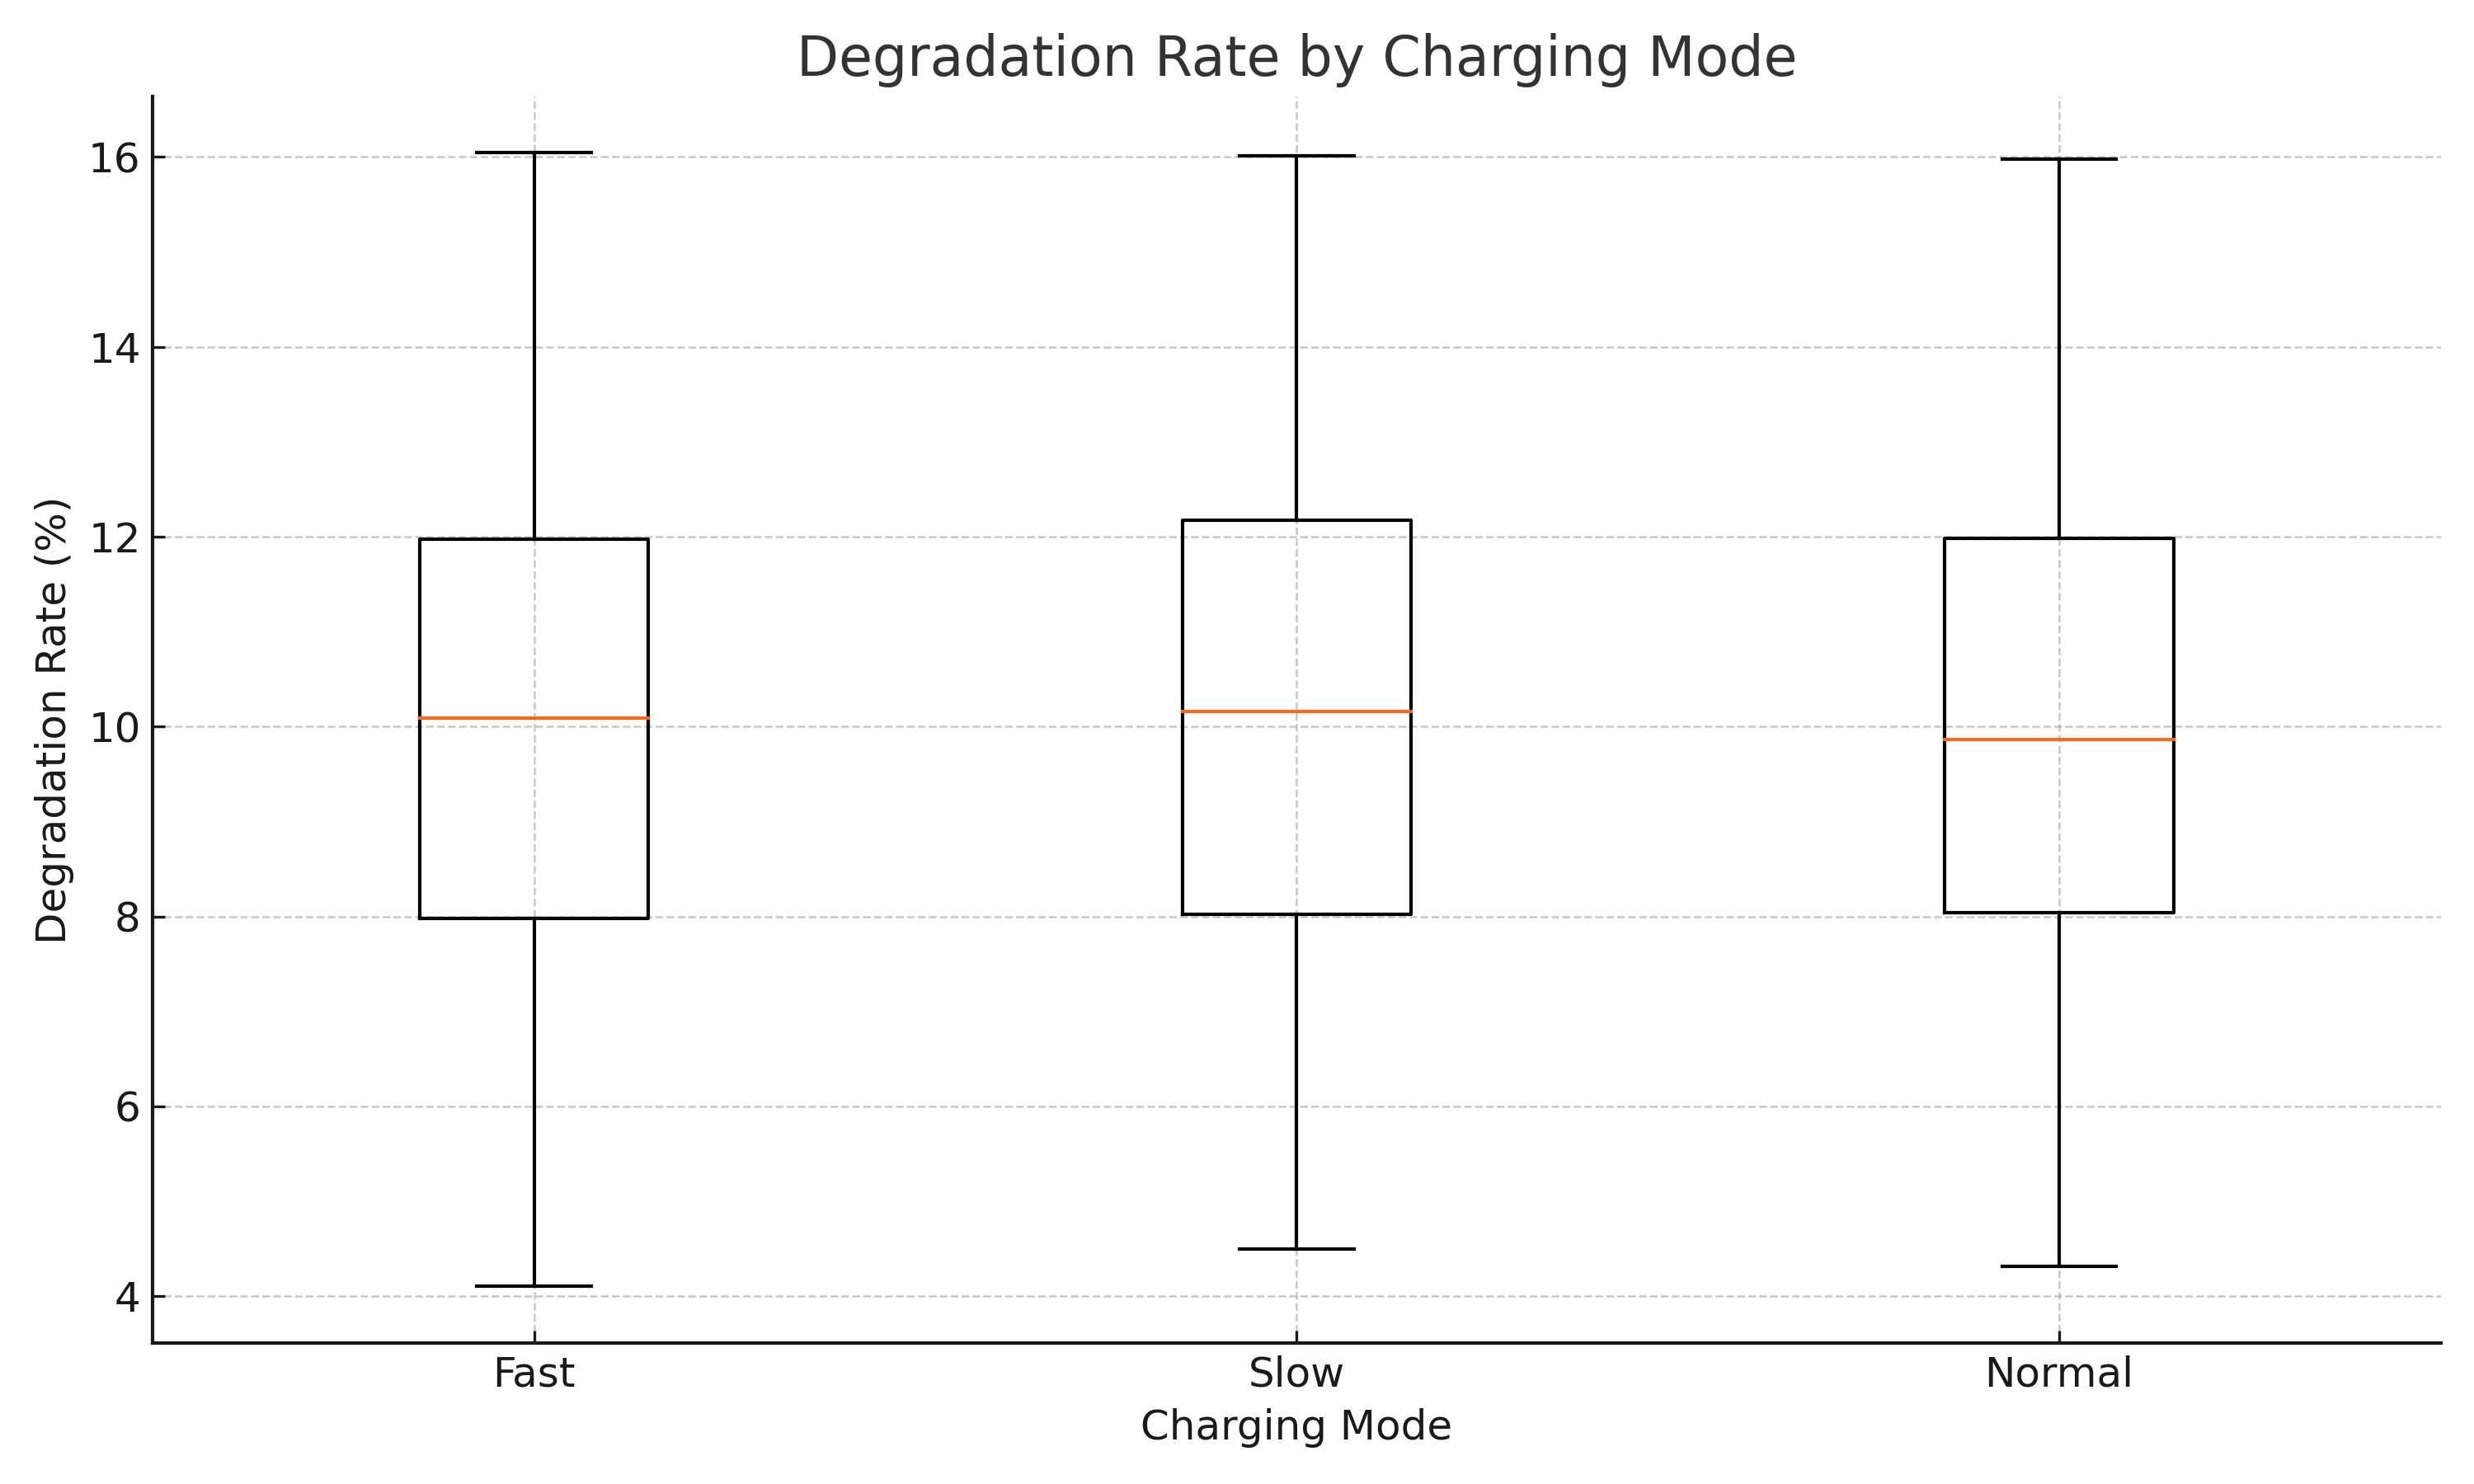
\includegraphics[width=0.7\textwidth]{fig_box_deg_mode.png}
 \caption{Degradation rate stratified by charging mode}
 \label{fig:mode}
\end{figure}

\begin{figure}[h]
 \centering
 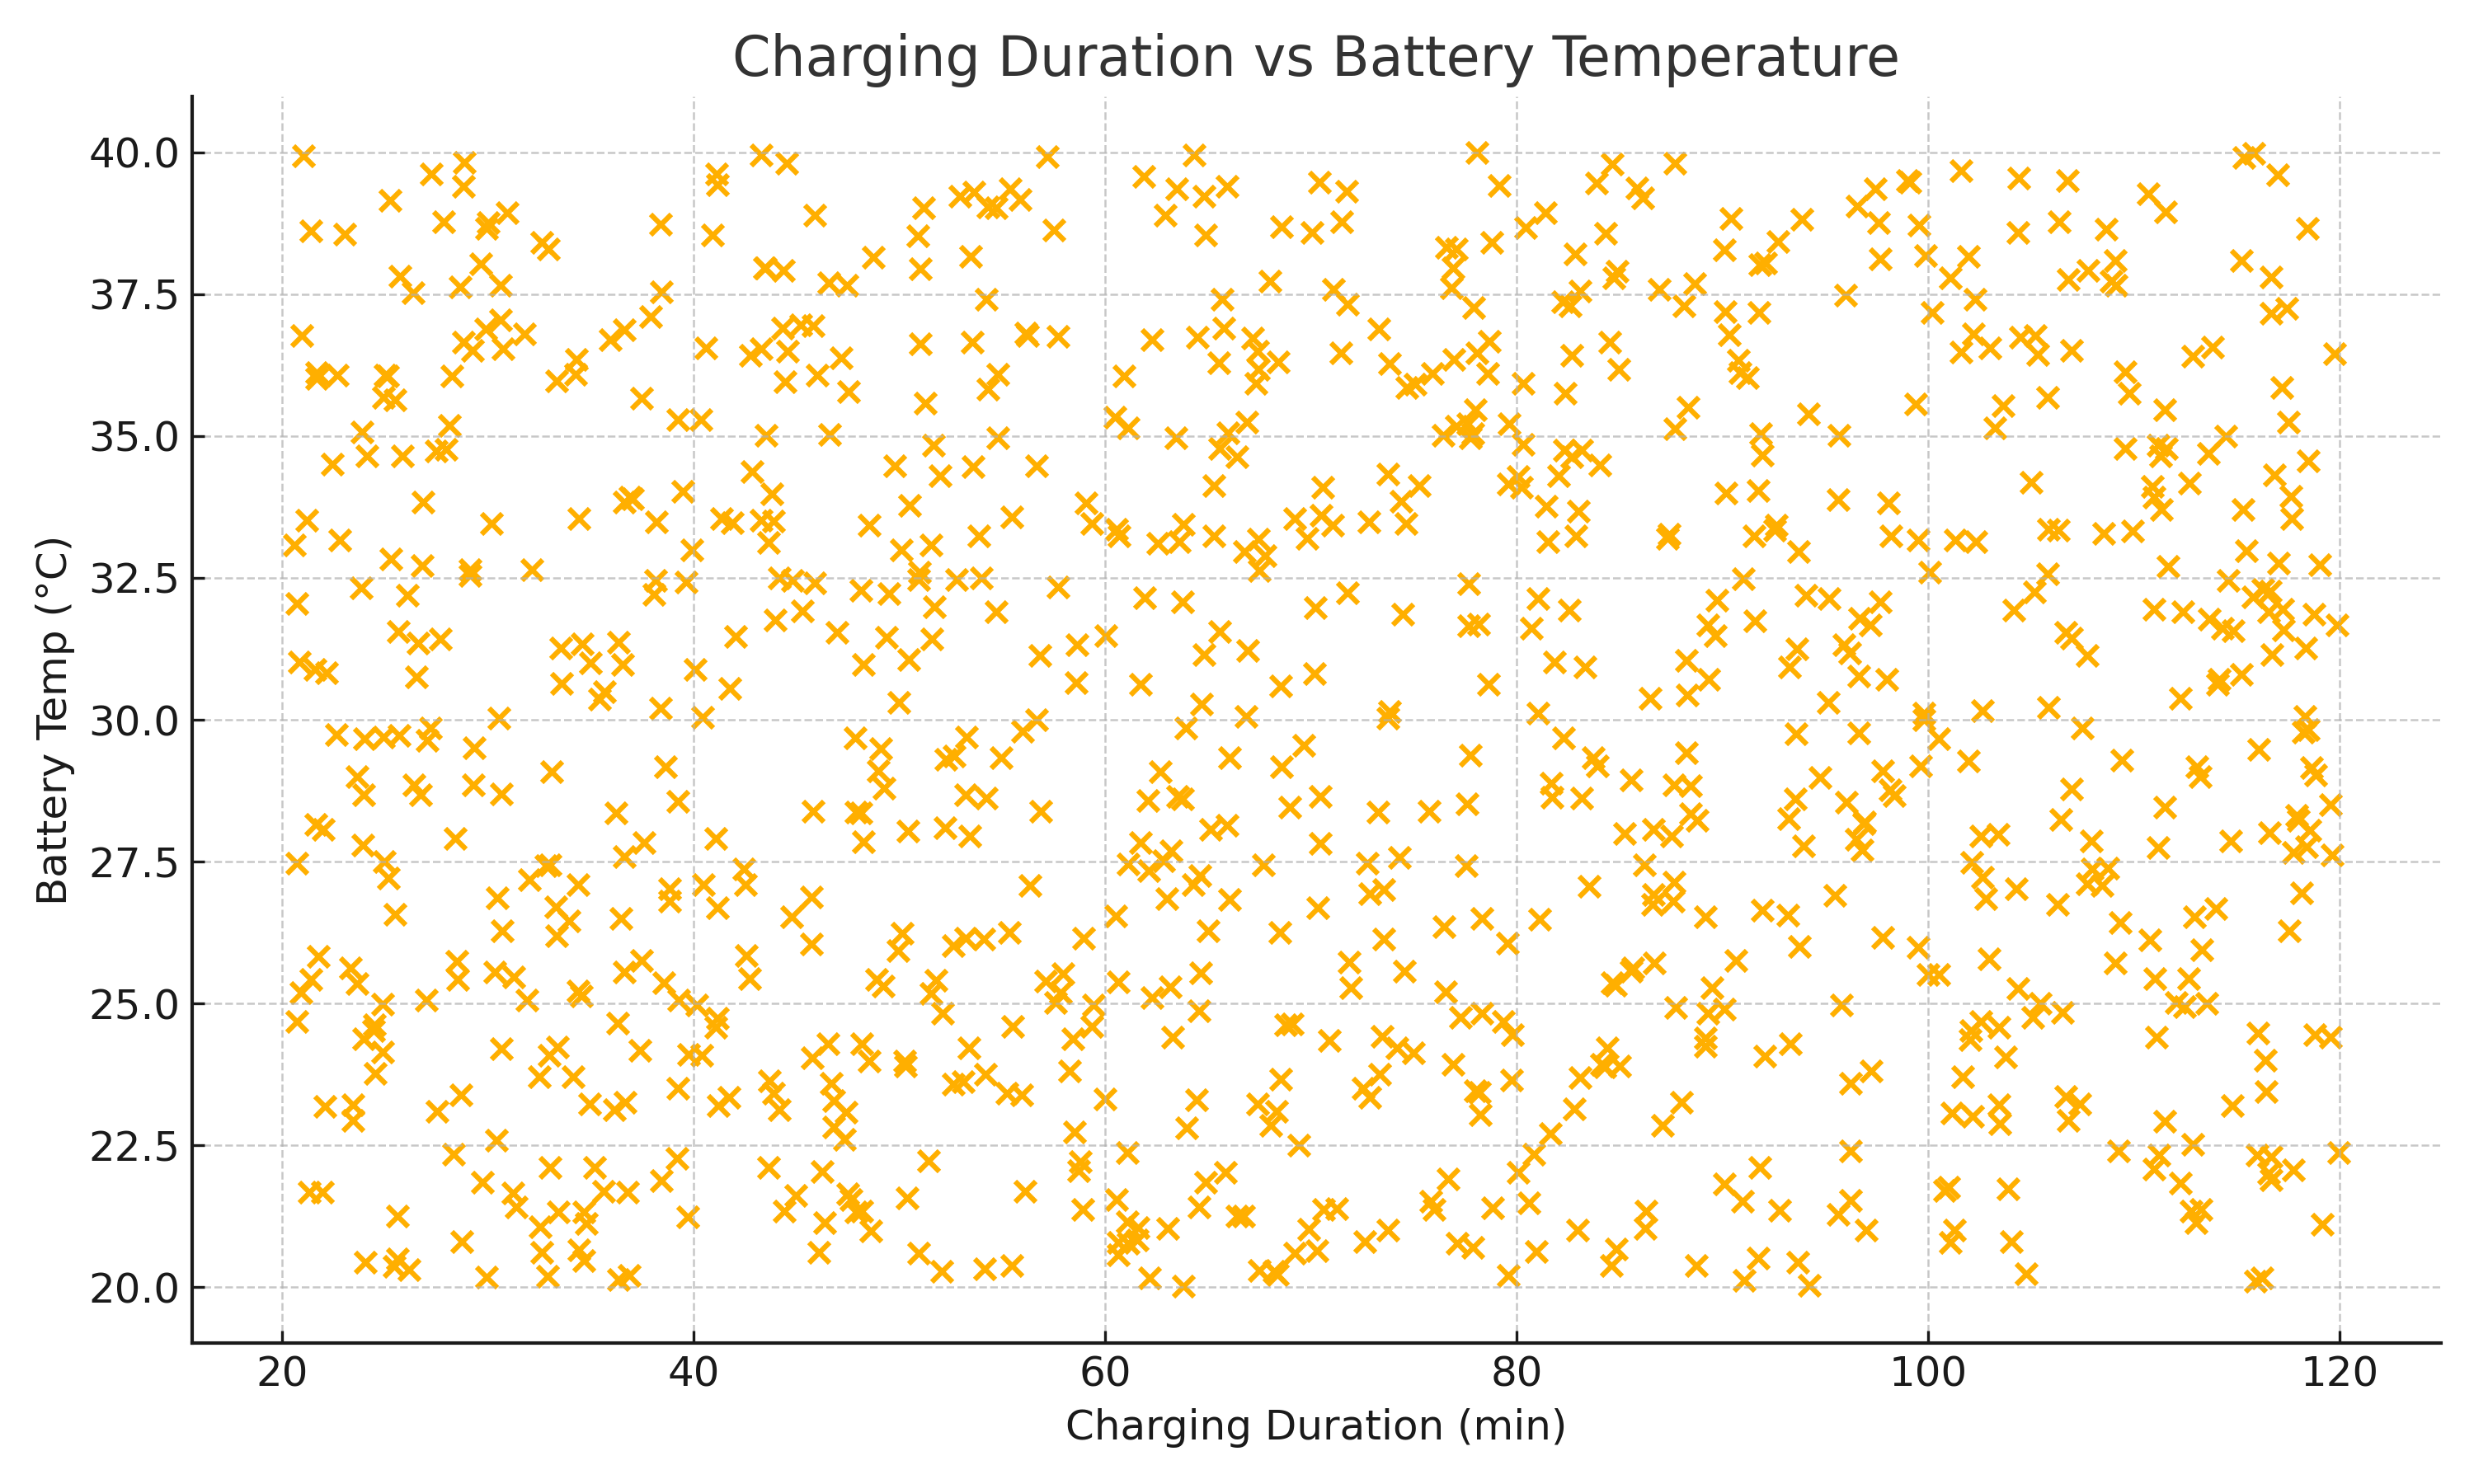
\includegraphics[width=0.7\textwidth]{fig_duration_temp.png}
 \caption{Session duration versus battery temperature}
 \label{fig:duration}
\end{figure}

\begin{figure}[h]
 \centering
 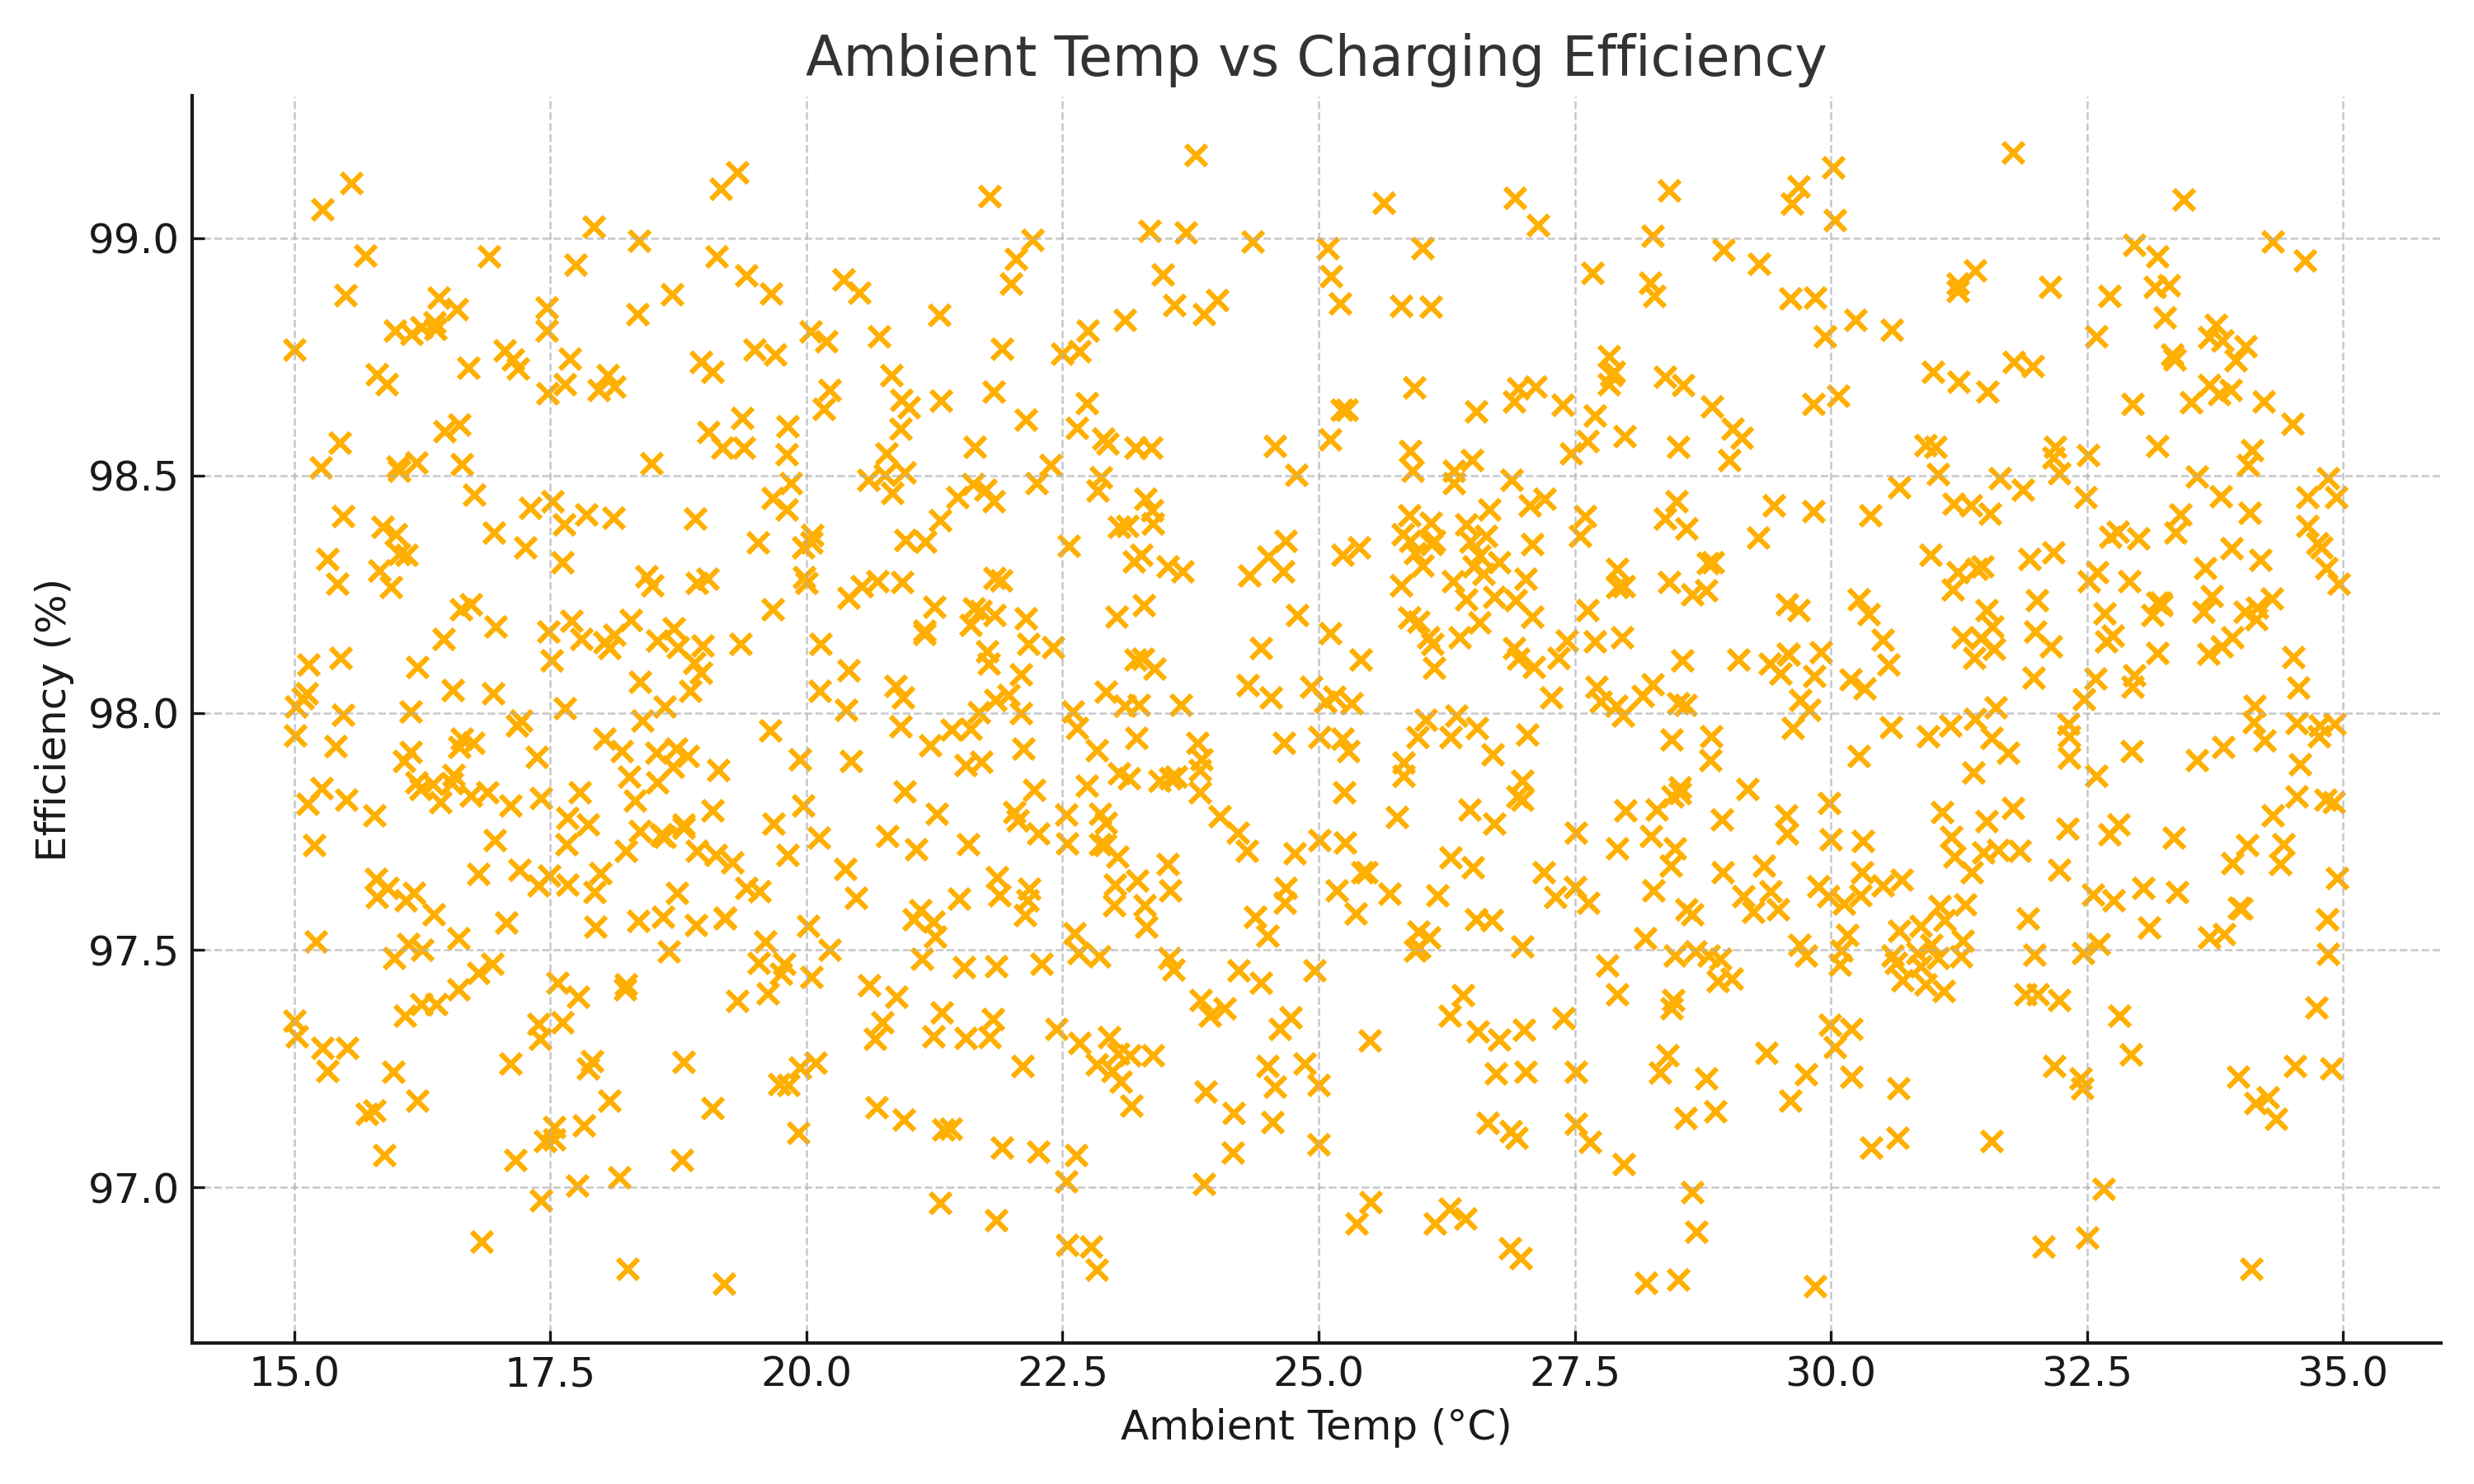
\includegraphics[width=0.7\textwidth]{fig_ambient_eff.png}
 \caption{Ambient temperature versus charging efficiency}
 \label{fig:ambient}
\end{figure}

\clearpage
\section{Correlation \& Multicollinearity}
The heatmap (Fig.~\ref{fig:heat}) shows a strong positive correlation between \textit{Charging Cycles} and \textit{Degradation Rate} ($r\,\approx\,0.85$).  
Variance Inflation Factor analysis confirmed limited multicollinearity (all VIF $<5$ except the cycles--degradation pair).

\section{Conclusion}
Key insights:\begin{itemize}
 \item Frequent cycling accelerates degradation; smart scheduling could extend battery life. 
 \item Extreme ambient temperatures reduce charging efficiency by up to 1\%.
 \item Most variables are weakly correlated, ensuring each contributes unique information for future predictive models.
\end{itemize}

The cleaned dataset and all figures included here support transparent, reproducible research into EV charging behaviour.

\end{document}
